Stoffe befinden sich in einem Aggregatzustand: flüssig, fest oder gasförmig.
Diese Zustände sind von zwei Freiheitsgraden abgängig, zum einen der Temperatur $T$,
und zum anderen von dem Druck $p$. Die Abhängigkeit dieser Größen wird klassicher
weise in einem Phasendiagramm dargestellt.

\begin{figure}   % {0.48\textwidth}
  \centering
  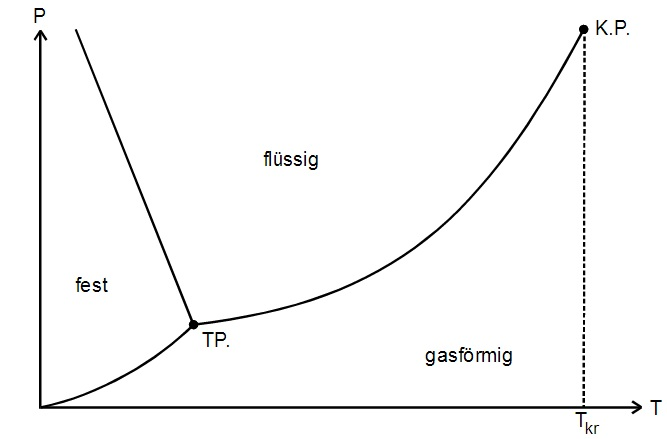
\includegraphics[height=5cm]{Zustandsdiagramm.jpeg}
  \caption{qualitatives Phasendiagramm des Wassers}
  \label{fig:phase}
\end{figure}

In diesem Phasendiagramm ist zu sehen, dass es zwei besondere Punkte gibt,
den Tripel-Punkt (T.P.) und den kritischen Punkt (K.P.). Am T.P. liegen alle drei
Phasen vor, am kritischen Punkt existieren zwei Phasen nebeneinander, wodurch
der Druck bei gegebener Temperatur durch die Dampfdruckkurve festgelegt ist.
Diese Kurve ist im wesentlichen von Verdampfungswärme $L$ abhängig. Sie beschreibt
die Energiemenge, die zur Umwandlung von einem Mol Flüssigkeit in Dampf benötigt wird,
bei gleicher Temperatur. Diese Größe ist temperaturabhängig.

Bei diesem Verdampfungsprozess erhöht sich die kinetische Energie der Teilchen,
welche nach der Maxwellschen Geschwindigkeitsverteilung bestimmt werden kann. Ist
ihre Energie groß genug, um die Van-der-Waals Kräfte zu überwinden, so können die
Teilchen die Flüssigkeitsoberfläche verlassen und in den gasförmigen Zustand übergehen.
Hierzu muss jedoch entweder Energie von außen hinzugefügt oder dem Wasser entzogen
werden, wodurch dieses abkühlt. Dieser Prozess ist reversibel. Die Verdampfungswärme
wird bei Kondensation somit wieder frei. Zwischen Verdampfung und Kondensation stellt
sich dann ein Gleichgewicht ein. Der hier herrschende Druck wird als Sättigungsdampfdruck
bezeichnet. Er hängt nicht vom Volumen des Gasraumes ab, wodurch die allgemeine
Gasgleichung
\begin{equation}
  pV = RT   \ ,\ mit \ R = allgemeine \ Gaskonstante \label{eq:ideal}
\end{equation}
nicht gilt.

Zur Berechnung der Dampfdruckkurve wird der reversible Kreisprozess von Wasser
zwischen Verdampfung und Kondensation betrachtet.

\begin{figure}
  \centering
  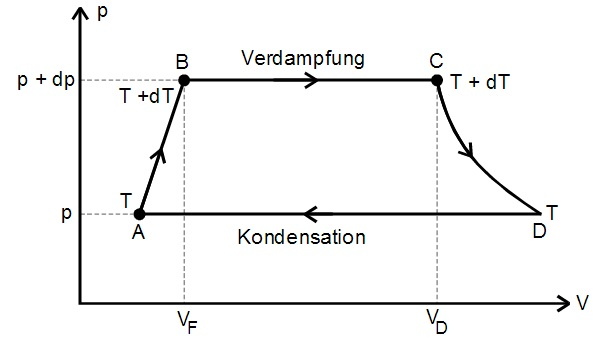
\includegraphics[height=4cm]{Kreisprozess.jpeg}
  \caption{reversibler Kreiprozess für Verdampfung und Kondensation}
  \label{fig:kreis}
\end{figure}

Zu Beginn ist der Stoff flüssig. Wird nun eine Wärmemenge $dQ$ hinzugefügt,
so erhöht sich der Druck, das Volumen und die Temperatur (A \rightarrow \ B).
Nun verdampft die Flüssigkeit isotherm und isobar, das Volumen
vergrößert sich weiterhin (B \rightarrow \ C). Jetzt gibt das Gas die erhöhte
Temperatur wieder auf, wodurch sich auch der Druck wieder senkt (C \rightarrow \ D).
Zuletzt gibt der Dampf die zugeführte Wärmeenergie wieder ab. Dies führt zu einer
isobaren und isothermen Kondensation (D \rightarrow \ A).
Wird nun die geleistete Arbeit mit den Wärmeenergien gleichgesetzt, so ergibt sich
folgende Gleichung:

\begin{equation}
  (C_F - C_D)dT + dL = (_D - V_F)dp .
\end{equation}

Nach dem zweiten Hauptsatz der Thermodynamik folgt für die Summe der Wärmemenge
in einem reversiblen Kreisprozess

\begin{equation}
  \sum_i{\frac{Q_i}{T_i}} = 0 . \notag
\end{equation}

Unter weiteren Vereinfachungen ergibt sich dann die Clausius-Clapeyronsche
Gleichung
\begin{equation}
  (V_D - V_F)dp = \frac{L}{T}dT .
\end{equation}

Liegt die Temperatur $T$ weit unter der kritischen Temperatur $T_{Kr}$, so können
folgende Näherungen angenommen werden:
\begin{itemize}
  \item $V_F$ ist gegenüber $V_D$ zu vernachlässigen \\
  \item $V_D$ gehorcht der idealen Gasgleichung (\ref{eq:ideal}) \\
  \item $L$ ist druck- und temperaturunabhängig \\
\end{itemize}

Daraus folgt dann

\begin{align}
  \ln{(p)} = -\frac{L}{RT} + \ln{(p_0)}  \ & bzw. \  % hier hätte ich gerne einen größeren Abstand
  P = p_0 \exp{\biggr(-\frac{L}{RT} \biggl)} .
\end{align}
